\lecdate{20.03.2017}
Problem: Aussagenlogik ist wenig mächtig.\\
Aussagen, die sich nicht formulieren lassen:
\begin{itemize}
\item „Alle Vögel können fliegen.“\\
(Nur formulierbar, wenn alle Vögel einzeln als Atomformeln beschrieben werden. Diese Formel der Aussagenlogik wäre dann allerdings sehr lang.)
\item „Wenn X eine Katze ist, dann ist X ein Haustier.“\\
(In der Aussagenlogik sind keine Variablen möglich.)
\item „Für jedes Land gibt es eine Hauptstadt.“
\end{itemize}

\section{Syntax der Prädikatenlogik}
\cparagraph{Definition}
Sei $V$ eine Menge von Variablen, $K$ eine Menge von Konstante und $F$ eine Menge von Funktionssymbolen.
\begin{itemize}
\item Dann sind alle Variablen $V$ und Konstanten in $K$ Terme.
\item Wenn $t_1, \dots, t_n$ Terme sind und $f$ ein $n$-stelliges Funktionssymbol ist, dann ist auch $f(t_1, \dots, t_n)$ ein Term. 
\end{itemize}

\cparagraph{Beispiel}
$V=\{x,y,z\},\; K=\{a,b,c\},\; F=\{+,*\}$. Terme sind $x,a,x+a,x*(x+1)$.

\cparagraph{Definition}
Sei eine Menge von Prädikatensymbolen gegeben. Die Formeln der Prädikatenlogik sind induktiv definiert:
\begin{itemize}
\item Wenn $t_1, \dots, t_n$ Term und $P$ ein Prädikatensymbol der Stelligkeit $n$ ist,\\ dann ist $P(t_1, \dots, t_n)$ eine Formel.
\item Sind $F,G$ Formeln, dann auch $F\wedge G, \; F\vee G,\; \neg F,\; (F)$.
\item Wenn $x$ eine Variable und $F$ eine Formel ist, dann sind auch $\forall x \,F, \; \exists x\,F$ Formeln.
\end{itemize}

\cparagraph{Bemerkung} Wie in der Aussagenlogik definiert sich $\to, \; \leftrightarrow$.\\
Vorrang der Operatoren: $\neg;\; \forall, \; \exists;\; \wedge, \; \vee;\; \to,\; \leftrightarrow$

\cparagraph{Beispiel}
\begin{itemize}
\item $\forall x\, (vogel(x) \to fliegt(x))$\\
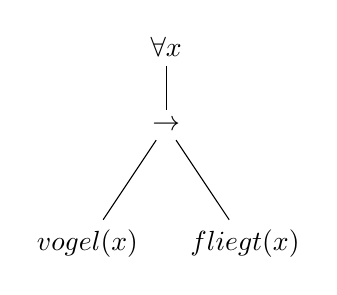
\begin{tikzpicture}
\node (v1) at (-0.5,2) {$\forall x$};
\node (v2) at (-0.5,1) {$\to$};
\node (v3) at (-1.5,-0.5) {$vogel(x)$};
\node (v4) at (0.5,-0.5) {$fliegt(x)$};
\draw (v1) -- (v2);
\draw (v2) -- (v3);
\draw (v2) -- (v4);
\end{tikzpicture}
\item $\forall x\, (katze(x) \to haustier(x))$
\item $\forall x\, (land(x) \to \exists y\, hauptstadt (x,y))$\\
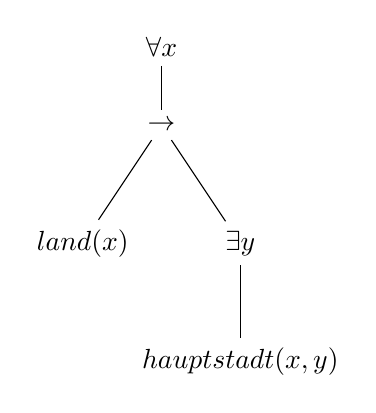
\begin{tikzpicture}
\node (v1) at (-0.5,2) {$\forall x$};
\node (v2) at (-0.5,1) {$\to$};
\node (v3) at (-1.5,-0.5) {$land(x)$};
\node (v4) at (0.5,-0.5) {$\exists y$};
\draw (v1) -- (v2);
\draw (v2) -- (v3);
\draw (v2) -- (v4);
\node (v5) at (0.5,-2) {$hauptstadt(x,y)$};
\draw (v4) -- (v5);
\end{tikzpicture}
\item $katz(feli)$ mit $feli \in K$
\end{itemize}

\section{Semantik der Prädikatenlogik (informal)}
Wir betrachten zunächst eine (unwichtige) Menge $U$ (Universum), die alle zu betrachtenden Objekte (Vögel, Katzen, Länder usw.) enthält. Davon betrachten wir Teilmengen, z.B. die Menge aller Vögel, Länder usw. sowie mehrstellige Relationen auf $U$ (z.B. Hauptstadt, verheiratet).

Beispiel: $Hauptstadt=\{(Berlin,\;Deutschland), (Paris, \; Frankreich)\} \subseteq \underbrace{U \times U}_{oder:\; Stadt\times Land}$\\
Den Prädikatensymbolen müssen Prädikate (Relationen) zugeordnet werden.

Beispiel: Ordnen dem Prädikatensymbol $vogel$ das Prädikat „Menge aller Vögel“ zu.\\
Dadurch ergibt sich der Wahrheitswert einer Formel: 
\begin{itemize}
\item Die Formel $P(t_1, \dots, t_n)$ ist wahr \gdw{} $(t_1, \dots, t_n) \in P$.
\item Die Wahrheit von $F\wedge G, \; F\vee G,\; \neg F$ ist wie in der Aussagenlogik definiert.
\item $\exists x \, F$ ist wahr \gdw{} es ein $x$ aus dem Universum gibt, mit dem $F$ wahr ist.
\item $\forall x \, F$ ist wahr \gdw{} $F$ für alle $x$ aus dem Universum wahr ist.
\end{itemize}
\cparagraph{Beispiel}
Sei $vogel=\{Amsel, Drossel, Fink, Star\}$\\
und $fliegt=vogel \cup \{Maikaefer, A380\}$
\begin{itemize}
\item $vogel(Amsel)$ ist wahr.
\item $vogel(Maikaefer)$ ist falsch.
\item $\exists x \, vogel(x)$ ist wahr.
\item $\forall x \, vogel(x)$ ist falsch.
\item $\forall x \,(vogel(x) \to fliegt(x))$ ist wahr.
\end{itemize}

\cparagraph{Beispiel} Sei $land=\{Deutschland, Frankreich\}$ und \\
$hauptstadt = \{ (Berlin, Deutschland), (Paris, Frankreich) \}$.\\
Für jedes Land gibt es eine Hauptstadt:
$$\forall x \,(land(x)\to \exists y \, hauptstadt(y,x))$$
\cparagraph{Beispiel}\lecdate{27.03.2017} Seien die Relationen $Katze$ (Menge aller Hauskatzen) sowie $Haustier$ (Menge aller Haustiere) gegeben.\\
Jede Katze ist ein Haustier:
$$\forall x \,(Katze (x) \to Haustier (x))$$
\cparagraph{Beispiel}
Seien $Mensch, \; Mann, \; Frau$ die Menge aller Menschen, Männer und Frauen.
\begin{itemize}
\item Jeder Mensch ist Mann oder Frau:
$$\forall x \, (Mensch(x) \to Mann(x) \vee Frau (x))$$
Anmerkung: wichtige Unterscheidung:\\
$Mensch(x) \to Mann(x) \vee Frau (x)$ liefert falsch zurück, wenn $x$ bspw. ein Stuhl -- das ist logisch richtig und \\
$Mensch(x) \wedge( Mann(x) \vee Frau (x))$ sagt, dass jedes $x$ entweder Mann oder Frau sein muss… ein Stuhl bspw. auch -- das ist falsch!
\item Jeder Mann und jede Frau ist ein Mensch:
$$\forall x \, (Mann(x) \vee Frau(x) \to Mensch(x))$$
Anmerkung: Obwohl im Satz „und“ steht, steht in der Prädikatenlogik das „oder“. Das „und“ ist in diesem Sinne gemeint:\\
$\forall x \, (Mann(x)\to Mensch(x)) \wedge \forall x\, (Frau(x) \to Mensch(x))$
\item Kein Mensch ist gleichzeitig Mann und Frau:
$$\forall x \, (Mensch(x) \to  \neg (Mann(x) \wedge Frau(x)))$$
\end{itemize}

\subsection{Rechenregeln}
\cparagraph{Definition}
\begin{itemize}
\item $\neg \forall x \, F \equiv \exists x\, \neg F$
\item $\neg \exists x \, F \equiv \forall x\, \neg F$
\item Für $Q \in \{\forall, \exists\}$ und $\circ \in \{ \wedge, \vee\}$ gilt:\\
$(Q x F ) \circ G \equiv Qx\,(F\circ G)$, falls $x$ in $G$ nicht frei vorkommt.
\item $\forall x \, F \wedge \forall x \, G \equiv \forall x (F \wedge G)$
\item $\exists x \, F \vee \exists x \, G \equiv \exists x \, (F \vee G)$
\item $\forall x \, \forall y \, F \equiv \forall y \, \forall x \, F$
\item $\exists x \, \exists y \, F \equiv \exists y \, \exists x \, F$
\end{itemize}

\cparagraph{Beispiel}
$(\exists x\,Katze(x)) \vee Vogel(y)\equiv \exists x \, (Katze (x) \vee Vogel(y))$

\subsection{Pränexform}
\cparagraph{Definition} Eine Aussage $F$ ist in \emph{bereinigter Pränexform}, wenn
$$F= Q_1 y_1 \,\dots\, Q_ny_nG$$
wobei $Q_i\in \{\forall, \exists\}$, $G$ keine Quantoren enthält und $y_1, \,\dots\,,\, y_n$ paarweise verschieden sind.\bigskip\\
Für jede Aussage $F$ gibt es eine äquivalente Formel im bereinigter Präexform.
\cparagraph{Beispiel}
\begin{align*}
&\forall x \, (land(x) \to \exists y \, hauptstadt(y,x))\\
\equiv \;&\forall x\, (\neg land(x) \vee \exists y\, hauptstadt(y,x))\\
\equiv \;&\forall x\, (\exists y \, (\neg land(x) \vee hauptstadt(y,x)))\\
\equiv \;&\forall x\, \exists y \, (land (x) \to hauptstadt(y,x))
\end{align*}
\cparagraph{Beispiel}
Nicht jeder Vogel fliegt:
\begin{align*}
&\neg \forall x \, (Vogel (x) \to fliegt(x))\\
\equiv \, & \forall x \, (\neg Vogel(x) \vee fliegt(x))\\
\equiv \, & \exists x \, \neg (\neg Vogel(x) \vee fliegt(x))\\
\equiv \, & \exists x \, (Vogel(x) \wedge \neg fliegt(x))
\end{align*}
(Nicht jeder Vogel fliegt. Durch Umformung erfährt man: Es muss einen Vogel geben, der nicht fliegt)\\
Achtung: Diese Formel sollte nicht wieder in die Implikation umgeformt werden, da sie sonst auch für bspw. einen Stuhl gültig wäre, was nicht gewollt ist: $\exists x (\neg Vogel(x) \to fliegt(x))$ (Stuhl ist kein Vogel, also fliegt er).
\subsection{Hornformeln}
\cparagraph{Definition}
\begin{itemize}
\item Ein \emph{Literal} ist eine Atomformel oder eine negierte Atomformel. Eine nicht negierte Atomformel nennt man \emph{positiv} (auch: Fakt), eine negierte \emph{negativ}. 
\item Eine Formel heißt \emph{Hornklausel}, wenn sie eine $\vee$-Verknüpfung von Literalen ist, von denen höchstens eins positiv ist.
\item Eine Hornformel ist eine $\wedge$-Verknüpfung von Hornklauseln.
\end{itemize}

\cparagraph{Beispiel}
\begin{itemize}
\item Literale: $P(x,y),\; \neg P(x,y), \; \neg Q(z *x+y)$
\item Hornklauseln: $\neg P(x,y) \vee Q(x),\; \neg P(x,y) \vee \neg Q (x), \; Q(x)$
\end{itemize}

\cparagraph{Wichtiger Spezialfall} Hornklauseln mit mindestens zwei Literalen und genau einem positiven Literal. Diese lassen sich als Folgerung darstellen, da
\begin{align*}
&\neg A_1 \vee \dots \vee A_{n-1}\vee A_n\\
\equiv\;& \neg (A_1 \wedge \dots \wedge A_{n-1})\vee A_n\\
\equiv\; & A_1 \wedge \dots \wedge A_{n-1} \to A_n
\end{align*}
Mit Hilfe von Hornklauseln lassen sich Regeln formulieren, z.B. $\forall x \, (Katz(x) \to Haustier(x))$ (die Klammer lässt sich, wie im Spezialfall gesehen, umformen [dieses Mal von der Folgerung zurück), ist sie eine Hornformel]).\\
Wenn diese Regeln mit $\wedge$ verknüpft werden, können diese zusammen mit Fakten (einzelnes positives Literal) als Wissensbasis betrachtet werden.\\
Die Wissenbasis ist dann eine Hornformel.

\cparagraph{Beispiel}\parskp
$katze(feli) \wedge \forall x \, (katze(x) \to haustier(x))$ ist eine Hornformel, die als einfache Wissensbasis betrachtet werden kann. Daraus lässt sich die Aussage dass Feli ein Haustier ist schließen, obwohl es nicht explizit dort steht. Das ist die Aufgabe eines Expertensystems.\\
Grundlegender Aufbau eines Expertensystems:
\begin{center}
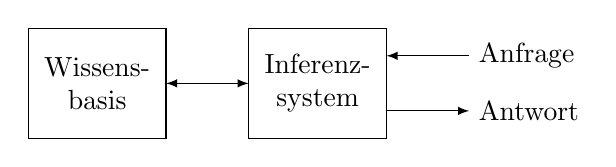
\begin{tikzpicture}[scale=.7]
\draw  (-3,3.5) rectangle (-0.5,1.5) node[pos=.5, align=center]{Wissens-\\basis};
\draw  (1,3.5) rectangle (3.5,1.5) node[pos=.5, align=center]{Inferenz-\\system};
\draw [latex-latex] (1,2.5) -- (-0.5,2.5);
\draw [-latex] (5,3) node[right]{Anfrage} -- (3.5,3);
\draw [-latex] (3.5,2) -- (5,2) node[right]{Antwort};
\end{tikzpicture}
\end{center}

\chapter{Prolog-Programmierung}
Prolog: Programming in Logic\\
Prolog-Programme sind im Wesentlichen Hornformeln, bei denen alle Variablen allquantisiert sind. Jede Klausel ist dabei eine Zeile eines Prolog-Programmes.

\cparagraph{Beispiel}$ $
\begin{lstlisting}[language=Prolog]
katze(feli).
haustier(X):-katze(X).
\end{lstlisting}
Dieses Prolog-Programm stellt die Hornformel $katze(feli) \wedge \forall x \, (katze(x) \to haustier(x))$ dar.\\
Anfrage an den Prolog-Interpreter:
\begin{lstlisting}[language=Prolog]
?-haustier(reni).
true.
\end{lstlisting}

\section{Syntax}
Prädikat: Wort in Kleinbuchstaben.\\
Konstante: Wort in Kleinbuchstaben.\\
(Bestimmung ob Prädikat oder Konstante erfolgt über die Position des Wortes: Konstanten treten immer in der Klammer von Prädikaten auf)\\
Variable: Wort, das mit einem Großbuchstaben beginnt.\\
"$\leftarrow$": ":-" (wird impliziert von).\\
"$\wedge$": ",".\\
Jede Klausel wird mit "." abgeschlossen. Alle Klauseln sind implizit mit $\wedge$ verknüpft.











